\documentclass{beamer}

\graphicspath{ {../dolgozat/images/} }
\usepackage[export]{adjustbox}
\usepackage{python}
\newcommand\tab[1][1cm]{\hspace*{#1}}

\usepackage{listings}
\usepackage{color}

% Code colorature
\definecolor{paszt}{RGB}{252,252,252}
\definecolor{keret}{RGB}{220,220,220}
\lstset{
backgroundcolor=\color{paszt},
% showlines=true,
framexleftmargin=4mm,
framexrightmargin=4mm,
framextopmargin=2mm,
framexbottommargin=2mm,
frameround=tttt,
frame=trbl,
rulecolor=\color{keret}
}

\usetheme{Copenhagen}
\useinnertheme{rectangles}

% ---- Mongo theme ----
%\definecolor{light-background}{RGB}{210,250,170}
%\definecolor{dark-background}{RGB}{128,92,64}
%\usecolortheme[RGB={220,250,180}]{structure}

% ---- Vanilla theme ----
% \definecolor{light-background}{RGB}{250,250,190}
% \definecolor{dark-background}{RGB}{128,92,64}
% \usecolortheme[RGB={210, 210, 140}]{structure}

% ---- Blue theme ----
%\definecolor{light-background}{RGB}{200,220,240}
%\definecolor{dark-background}{RGB}{100,110,120}
%\usecolortheme[RGB={180, 200, 230}]{structure}

% ---- Green theme ----
\definecolor{light-background}{RGB}{229,237,204}
\definecolor{dark-background}{RGB}{156,163,140}
\usecolortheme[RGB={180, 210, 150}]{structure}

\setbeamercolor{palette primary}{fg=black, bg=light-background}
\setbeamercolor{palette quaternary}{fg=white,bg=dark-background}

\setbeamercolor{title}{fg=black}
\setbeamercolor{frametitle}{fg=black}

% Set font
\usefonttheme{structurebold}

\frenchspacing

% Language packages
\usepackage[utf8]{inputenc}
\usepackage[T1]{fontenc}
\usepackage[magyar]{babel}

% AMS
\usepackage{amssymb,amsmath}

% Graphic packages
\usepackage{graphicx}

% Syntax highlighting
% \usepackage{listings}

\usepackage{tikz}

%\begin{figure}[htb]
%\begin{center}
%	\includegraphics[scale=0.4]{ps_times.png}
%\end{center}
%\end{figure}

% ==============
\begin{document}
% ==============

\title[Kínai karakterek felismerése, konvolúciós ANN]{
{\Large Kínai karakterek felismerése konvolúciós neurális
hálók használatával}
}
\author[Szilvási Péter]{\Large Szilvási Péter}
\date{Miskolci Egyetem, 2019. január 24.}

% --------------------
% Title page
\frame{\titlepage}

% --------------------
\begin{frame}[fragile]
\frametitle{Kínai karakterek felismerése}

\begin{tabular}{c c}
{\large Vonások, vonás sorrend} & 
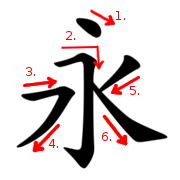
\includegraphics[scale=0.3, center]{vonasrend_ordered}
\end{tabular}

\begin{enumerate}
\item A vízszintes vonások megelőzik a függőleges vonásokat.
\item A balra lejtő vonások megelőzik a jobbra lejtő vonásokat.
\item Az írásjegyek írását felülről kell kezdeni.
\item Az írásjegyet balról jobbra haladva építik fel.
\item A felülről keretezett írásjegyeknél előbb a keretet kell meghúzni.
\item Az alulról keretezett írásjegyeknél a keretet legvégül kell meghúzni.
\item A teljes keretet mindig legvégül kell bezárni.
\end{enumerate}

\end{frame}

% --------------------
\begin{frame}[fragile]
\frametitle{OCR megvalósítások}

\begin{itemize}
\item Dokumentumok digitalizálása
\item OCR részei: szkennelő fej + szoftver [1]
\item Feldolgozási szintek: [2]
\begin{itemize}
	\item Alacsony szintű: zajos kép $\rightarrow$ előfeldolgozás $\rightarrow$ javított kép
	\item Középső szintű: kép $\rightarrow$ szegmentálás $\rightarrow$ kép jellemzők
	\item Magas szintű: jellemzők $\rightarrow$ osztályozás $\rightarrow$ osztálycímke
\end{itemize}
\end{itemize}

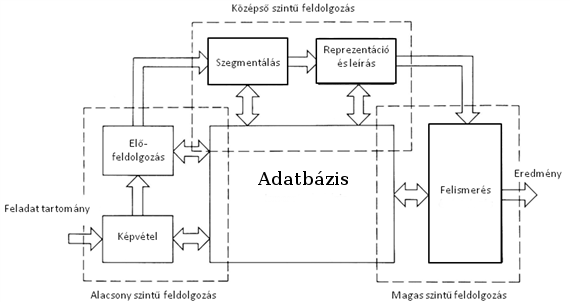
\includegraphics[scale=0.45, center]{ocr}

% Karakterek részekre bontása, struktúrális elemzése

% Betűtípusokból való eltérések

\end{frame}

% --------------------
\begin{frame}[fragile]
\frametitle{OCR megvalósítások}

OCR típusok: \textit{online}, \textit{offline} [3]

\bigskip

{\large Kínai karakter felismerése}
\begin{itemize}
\item Zaj szűrés: pontszerű zajok, elmosódás, forgatás, kontraszt
\item Jellemzők kinyerése
\end{itemize}
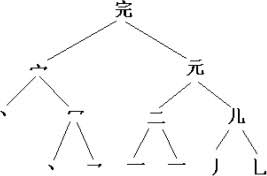
\includegraphics[scale=0.6, center]{ocr_features}

\end{frame}

% --------------------
\begin{frame}[fragile]
\frametitle{OCR megvalósítások}
\begin{tabular}{c c}
{\large Egy elterjedt algoritmus [4]} & 

\includegraphics[scale=0.2, center]{chinese_fonts1}
\end{tabular}
\begin{itemize}
\item Dimenzió redukció

\(d_i = \dfrac{l_i}{\sqrt{\displaystyle \sum_{k=1}^8 l_k^2}}\)
\begin{tabular}{ c c }
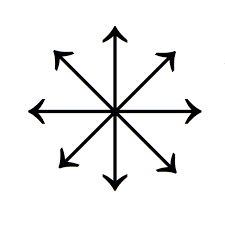
\includegraphics[scale=0.3]{8direction} & 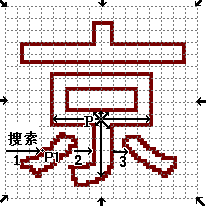
\includegraphics[scale=0.3]{ocr_PDC}
\end{tabular}
\item Tanítás
\item Tesztelés 
\begin{table}
\centering
\begin{tabular}{ |c|c|c|c|c|}
\hline
Font & Song & Fang & Kai & Hei\\
\hline
Train & 99.82 & 99.64 & 99.81 & 99.57\\
\hline
Test & 99.71 & 99.50 & 99.80 & 99.09\\
\hline
\end{tabular}
\end{table}
\end{itemize}
\end{frame}

% --------------------
\begin{frame}[fragile]
\frametitle{Jellemzők kinyerése, Dimenzió redukció}

\begin{itemize}
\item Főkomponens analízis (\textit{Principle Component Analysis})
\item Kernelek alkalmazása
\item Neurális háló szerkezete
\end{itemize}

\end{frame}

% --------------------
\begin{frame}[fragile]
\frametitle{Alacsony szintű jellemzők}

\begin{itemize}
\item Éldetektálás
\item Sarokérzékelés
\item Skála invariáns jellemző transzformáció (SIFT, \textit{Scale Invariant Feature Transform})
\end{itemize}

\end{frame}

% --------------------
\begin{frame}[fragile]
\frametitle{Irány szerinti jellemző kinyerés}

\begin{itemize}
\item Irány dekompozíció
\item Elmosódás és mintavétel
\item Számítási idők
\item Korlátozás nélküli minták
\end{itemize}

\end{frame}

% --------------------
\begin{frame}[fragile]
\frametitle{Mesterséges neurális hálók}

Neurális hálózatok [5]
\begin{itemize}
\item Rétegek
\item Elemei
\end{itemize}

Backpropagation
\begin{itemize}
\item Hiba $E_{total} = \sum \dfrac{1}{2}(target - output)^2.$
\item Láncszabály $\frac{\partial E_{total}}{\partial w_{5}} = \frac{\partial E_{total}}{\partial out_{o1}} \cdot \frac{\partial out_{o1}}{\partial net_{o1}} \cdot \frac{\partial net_{o1}}{\partial w_{5}}.$
\end{itemize}

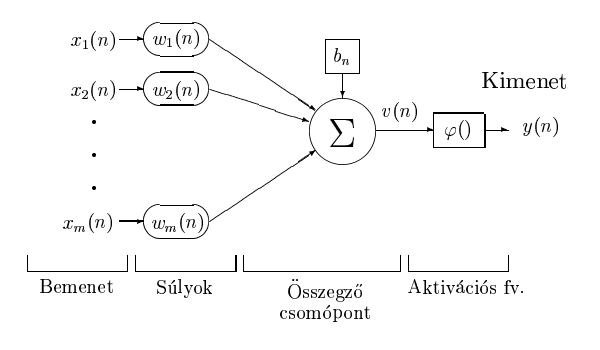
\includegraphics[scale=0.4, center]{ANNParts}

\end{frame}

% --------------------
\begin{frame}[fragile]
\frametitle{Konvolúciós neurális háló}
% A hálózat architektúrája, használt topológia
\begin{itemize}
\item Hálózat felépítése (konvolúciós rétegek $\rightarrow$ hagyományos ANN)
\item Bemenet $\rightarrow$ (\textit{Konvolúció $\rightarrow$ RELU $\rightarrow$ POOL}) $\rightarrow$ Kimenet(FC)
\end{itemize}
\begin{tabular}{c c}
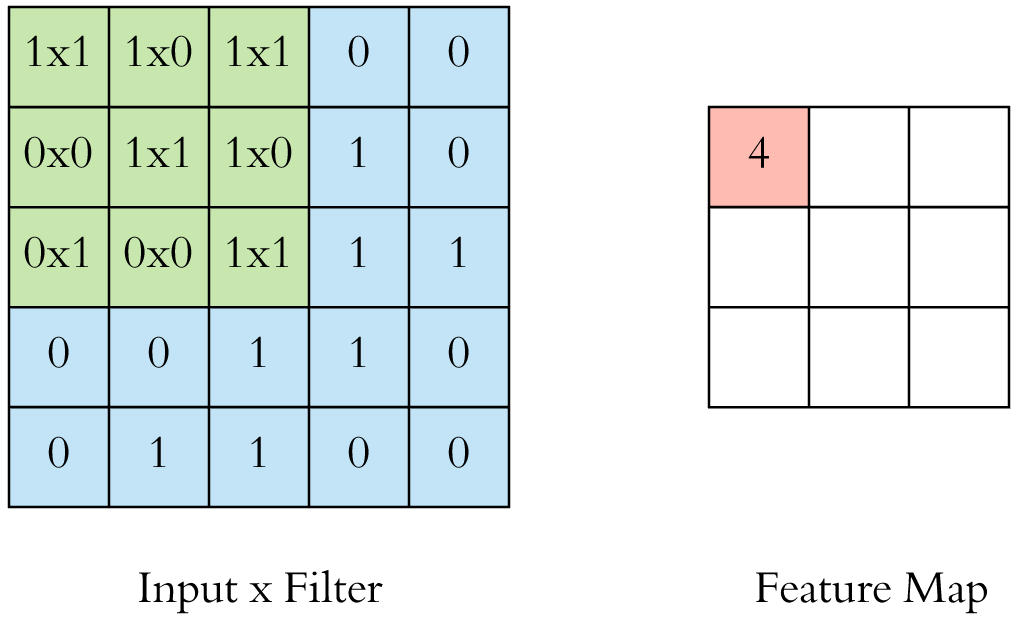
\includegraphics[scale=0.15]{convolution} & 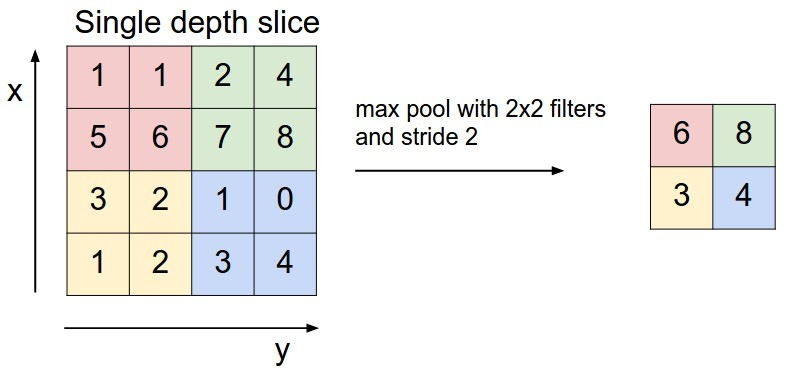
\includegraphics[scale=0.2]{maxpool}
\end{tabular}
\begin{itemize}
\item Hálózat tanítás
\end{itemize}
\begin{table}
\centering
\begin{tabular}{l l}
	1. Előre terjesztés & 3. Hiba visszaterjesztés\\
	2. Veszteség számítás & 4. Súly frissítés
\end{tabular}
\end{table}
\begin{itemize}
\item Dropout
\end{itemize}
\end{frame}

% --------------------
\begin{frame}[fragile]
\frametitle{A háló felépítése}

% 4.10-es ábra
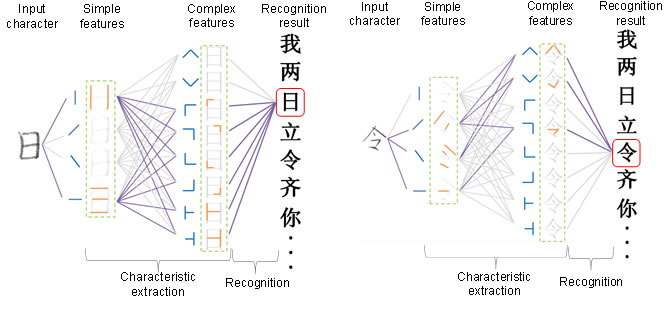
\includegraphics[scale=0.485]{CNN_CCR_working}

\begin{itemize}
\item Tesztelés
\item Transfer learning
\end{itemize}

\end{frame}

% --------------------
\begin{frame}[fragile]
\frametitle{A hálózat architektúrája}

% 5.2 ábra
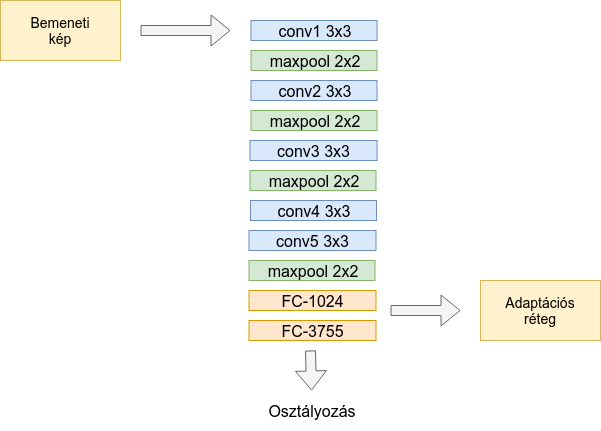
\includegraphics[scale=0.5]{architecture}

\end{frame}

% --------------------
\begin{frame}[fragile]
\frametitle{A hálózat architektúrája}

\begin{lstlisting}
model.add(
Convolution2D(1,	# filter retegek szama    
              3, 3,	# 3x3 kernel meret 
              strides=(1,1) # lepes
              input_shape=image))
\end{lstlisting}
\begin{lstlisting}
model.add(MaxPooling2D(pool_size=(2,2)))
\end{lstlisting}
\begin{lstlisting}
model.compile(loss='mean_squared_error', # Hiba
optimizer='adam', metrics=['accuracy'])

model.fit_generator(generator=training_data,
steps_per_epoch=1000, epochs=10)	# Tanitas
\end{lstlisting}

\end{frame}

% --------------------
\begin{frame}[fragile]
\frametitle{Az offline adatbázis}

Adathalmaz: nyomtatott, kézzel írott, generált

\medskip

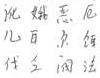
\includegraphics[scale=1.5, center]{offline_dataset4x3}

\begin{itemize}
\item Tanító/Teszt(80/20), \texttt{random.shuffle(self.images)}
\item Tanító minták változatossága
\item Tesztelés módja
\item Helyesség ellenőrzése
\end{itemize}

\end{frame}

% --------------------
\begin{frame}[fragile]
\frametitle{A felismerés hatékonysága}

% Eredmények konkrét százalékokkal
\begin{table}
\begin{tabular}{l c c}
0\%\tab $\rightarrow$\tab & 
\includegraphics[scale=0.5]{original} & \tab $\rightarrow$\tab 90-95\% \\
75-80\%\tab $\rightarrow$\tab & 
\includegraphics[scale=0.5]{noise} & \tab $\rightarrow$\tab 84\% \\
 68\%\tab $\rightarrow$\tab & 
\includegraphics[scale=0.5]{rotate} & \tab $\rightarrow$\tab 75\% \\
 87\%\tab $\rightarrow$\tab & 
\includegraphics[scale=0.5]{blur} & \tab $\rightarrow$\tab 93\% \\
\end{tabular}
\end{table}

\end{frame}

% --------------------
\begin{frame}[fragile]
\frametitle{Összegzés}
\begin{itemize}
\item Kínai karakterek
	\begin{itemize}
	\item stroke
	\item vonásrend
	\end{itemize}
\item OCR
	\begin{itemize}
	\item részei
	\item használt OCR bemutatás
	\end{itemize}
\item Jellemzők kinyerése
	\begin{itemize}
	\item dimenzió redukció
	\item alacsony szintű jellemzők
	\item irány szerinti jellemző kinyerés
	\end{itemize}
\item Neurális hálózatok
	\begin{itemize}
	\item hagyományos neurális háló (ANN)
	\item konvolúciós neurális háló (CNN)
	\end{itemize}
\item Validáció
	\begin{itemize}
	\item adathalmaz előállítás
	\item hálózat osztályozása
	\end{itemize}
\end{itemize}

\end{frame}

% --------------------
\begin{frame}[fragile]
\frametitle{Hivatkozások}

% \begin{thebibliography}{9}

\begin{itemize}

\item[1] Tikk Domonkos: \textit{Optikai karakterfelismerés}, online melléklet, TypoTeX kiadó, 2006.

\smallskip

\item[2] Rövid A., Vámossy Z., Sergyán S.: \textit{A gépi látás és képfeldolgozás párhuzamos modelljei és algoritmusai}, 2014.

\smallskip

\item[3] Liu, Yin, Wang, Wang: \textit{Online and offline handwritten chinese character recognition: benchmarking on new databases}, Pattern Recognition, 2013.

\smallskip

\item[4] X. Wu, M. Wu: \textit{A recognition algorithm for chinese characters in diverse fonts}, Image Processing, 2002.

\smallskip

\item[5] Fazekas István: \textit{Neurális hálózatok}, Debreceni Egyetem, 2013.

\end{itemize}

% \end{thebibliography}

\end{frame}

% --------------------
\begin{frame}[fragile]
    \frametitle{\ }

\begin{center}
\Large \textbf{Köszönöm szépen a figyelmet!}
\end{center}

\end{frame}

\end{document}
